% Chapter Template

\chapter{PID Gain Optimization} % Main chapter title

\label{Chapter7} % Change X to a consecutive number; for referencing this chapter elsewhere, use \ref{ChapterX}

\lhead{Chapter 7. \emph{PID Gain Optimization}} % Change X to a consecutive number; this is for the header on each page - perhaps a shortened title

%----------------------------------------------------------------------------------------

In order to arrive at a solution to the quad-rotor energy optimization problem that is closer to running in real-time, a heuristic approach has been adopted. Recall that our general aim is to effectively control the vector position of the quad-rotor and additionally use the least energy in doing so. The relative simplicity of a PID controller makes it a good choice instead of the full nonlinear classical optimal control formulation. Also, if the PID control expressions are tuned well and that tuning is not changed, the control algorithm performs well.

The motivation for our heuristic method is to find the PID controller tuning which uses the least energy to drive the UAV to the desired state. The PID tuning defines the dynamics of the controller. Using the quad-rotor model derived in chapter 3, the performance of the controller and the dynamics of the system can be evaluated as a function of the tuning. Mathematically, this can be represented as follows.

The aim of the optimization is to find: $ argmin \big[  \sum_{k,i} \omega_i[k] \text{ } | \text{ } K_p , K_i , K_d  \big]  $ , where $\omega_i[k]$ is the $ith$ rotor speed at the $kth$ time step. The variables $K_p$ , $K_i$ and $K_d$ are the vectors of proportional, integral, and derivative gains defined as:

\begin{center}
$ K_p = \left[ \begin{array}{c} k_{px} \\ k_{py} \\ k_{pz}  \end{array} \right] , K_i = \left[ \begin{array}{c} k_{ix} \\ k_{iy} \\ k_{iz}  \end{array} \right], K_d = \left[ \begin{array}{c} k_{dx} \\ k_{dy} \\ k_{dz}  \end{array} \right] $
\end{center}

In our simulations, the time integral of all four motor speeds is proportional to the total energy used. Calculation of the actual energy used by the UAV in traversing a flight path would require a model for the motor. This is seen as unnecessary for our purposes since the time integral of the motor speeds and the total energy used will have the same effective minimum. Since the control input is calculated as part of the control algorithm anyway, it is used as a performance metric.


In any realistic application of UAV technology, the energy budget is only one important aspect of the control problem. Other important criteria for evaluating the performance of a controller are over-shoot of the desired location, the time of flight, and mathematical resonances or marginal instabilities. These factors must be considered in the design of the system. However, in the initial results described below, the time integral of the motor speeds is used as a single performance metric. The reason for this is to simplify the relationship between the performance metric and the PID gains. This is described in the next section.


\section{Initial Simulation Results}

In the context of the optimization process described in the previous section, there is evidence for the lack of robustness of the PID control. This can be shown by analyzing the relationship between the measured total thrust and the PID gains. Ideally, a gradient descent method would be used to minimize the thrust as a function of the control gains. The basic flow of the algorithm that we would really like to implement is as follows.


\begin{enumerate}
\item Choose a set of proportional and derivative gains for each vector direction (x,y, and,z),
\item Perform a simulation that controls the quad-rotor from an initial vector position to a desired vector position
\item Calculate the sum of the four motor speeds over the duration of the simulation
\item Appropriately change the PID gains such that the sum of the motor speeds decreases
\item Go to step 1. Repeat until the sum of the motor speeds is found to be a minimum.
\end{enumerate}

In reality, is has been found that the relationship between the measured total thrust and PID gains is not well behaved. After many days of trying to debug a gradient descent algorithm, and observing inconsistent behavior, it was decided that a brute force method might be the only possibility. A deeper understanding of the objective function was needed. The brute force method simply requires that we simulate the system and determine the value of the performance criteria for each possible set of PID gain vectors within a given range.

In order limit the number of simulations required to really represent the dynamics of the system, the set point $(0,0,1)$ was chosen. By choosing this set point, the motion of the quad-rotor is intentionally limited to the z-direction which limits the number of possible gain vectors for this test. This makes the tuning of the $x$ and $y$ direction controllers irrelevant. To further limit the number of simulations required, the Ziegler-Nichols PID tuning method was used. This method is discussed in \cite{ziegler1942optimum}. There are also excellent resources online to explain tuning \cite{znwiki}.

The Ziegler-Nichols method specifies simple algebraic relationships between the proportional, integral, and derivative gains. This allows each of the PID gains to be expressed as a function of a single gain variable, $k_u$ , which is allowed to range from 1 to 100.




 The results of these simulations are shown in Figure \ref{fig:ku vs thrust}.


\begin{figure}[htbp]
	\centering
		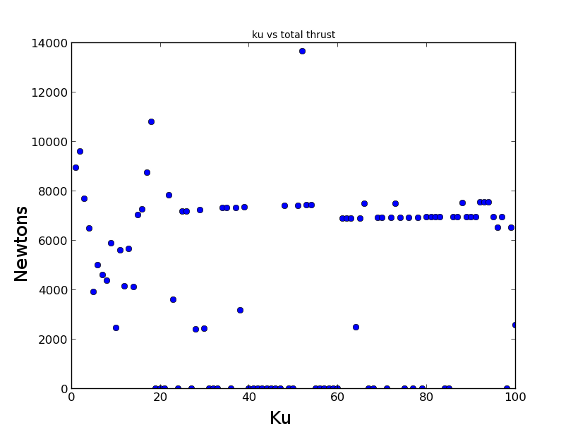
\includegraphics{Figures/kuvsthrust.png}
		\rule{35em}{0.5pt}
	\caption[Ku vs Thrust]{The relationship between Ku and the measured total thrust.}
	\label{fig:Ku vs Thrust}
\end{figure}

The relationship between Ku and the total measured thrust depicted in Figure \ref{fig:ku vs thrust} is rather disappointing to say the least. The values of zero total thrust are the result of simulations that failed to converge to the set point. Without an objective function that is at least marginally well behaved we have no hope to employ a gradient descent minimization technique. The relationship shown in Figure \ref{fig:ku vs thrust} is indeed a product of a deterministic system but displays little to no continuity. There are a few outliers in the data which are substantially lower in measured total thrust but the reason for their presence in the data as outliers is glib.

Another detail which cannot be ignored is that the total thrust alone is not sufficient as a performance criteria. Additionally, for appropriate control of the UAV,  the overshoot and oscillations which show up in improperly tuned PID controllers must be accounted for. Specifically, as the proportional gain is increased to drive the system to the desired location more quickly, the total thrust for the simulation will decrease but eventually the overshoot and oscillations grow to unacceptable levels. In the opposite fashion, if the differential gain is increased, the overshoot and oscillations will be suppressed but the time required to reach the set point will increase along with the total thrust. The competitive nature of these three (necessary) performance criteria further complicate the relationship between the PID gain vectors and the objective function making a gradient descent minimization technique even less viable.


\section{Brute Force Simulation Results}

Given that a standard mathematical optimization technique is out of the question, what options are left? With another year of research, a nonlinear control law could be implemented and would perhaps make the optimization possible, but this is uncertain. Sadly a naive, brute force approach is actually \textit{MORE} time efficient when compared to another year of research! For the sake of learning, a brute force algorithm is not so valuable. However, another year of research is simply not an option.

The decision was thus made to simply try many (many) possible gain vectors and have an appropriate objective function to characterize each of the simulations. Given that  the brute force algorithm is easy to write (and massively parallel-izable), around 6000 simulations were performed over a period of several hours. The computation was delegated two six independent instantiations of a python script, each one taking on a subset of the possible gain vectors and a separate CPU.

A separate script was used to parse through all the results of the simulations which were stored in many time-stamped files. Of the roughly 6000 simulations, about 1000 of them ran to completion without a numerical explosion. For these, the set point was reached and the stopping criteria for the simulation were satisfied. Of the 1000 or so good runs, about 80 simulations satisfied the maximum overshoot and oscillation criteria. Only the gain vectors which produced less than ten percent overshoot were accepted. Likewise, only simulations which crossed the desired set point in each direction fewer than four times were deemed acceptable. The remaining 80 simulations were sorted lowest to highest by total measured thrust. The optimal run that was found is detailed in Table \ref{table:optimalrun}. In Figures \ref{fig:optimal run 3D path} and \ref{fig:optimal run time domain} the dynamics of the system with optimal PID tuning are shown.


\begin{table}\label{table:optimalrun}
\begin{doublespace}
\centering
\begin{tabular}{l l}
The Optimal Run      \\
\hline
kpx                 & 15 \\
kpy                 & 15 \\
kpz                 & 40 \\
kix                 & 0.8 \\
kiy                 & 0.8 \\
kiz                 & 15 \\
kdx                 & 10 \\
kdy                 & 10 \\
kdz                 & 50 \\
ending iteration    & 987 \\
discrete time step   & 0.01 (s)\\
flight time         & 9.87 (s) \\
cpu runtime         & 11.41 (s)\\
return value        & 1 (great success)\\
initial position    & [0, 0, 1] (m)\\
set point           & [1, 1, 2] (m) \\
total thrust        & 4969.8 (Newton seconds) \\
x crossings         & 3 \\
x overshoot         & 0.0249 (m) \\
y crossings         & 1 \\
y overshoot         & 0.0185 (m)\\
z crossings         & 1 \\
z overshoot         & 0.0992 (m) \\
\end{tabular}
\end{doublespace}
\end{table}

\begin{figure}[htbp]
	\centering
		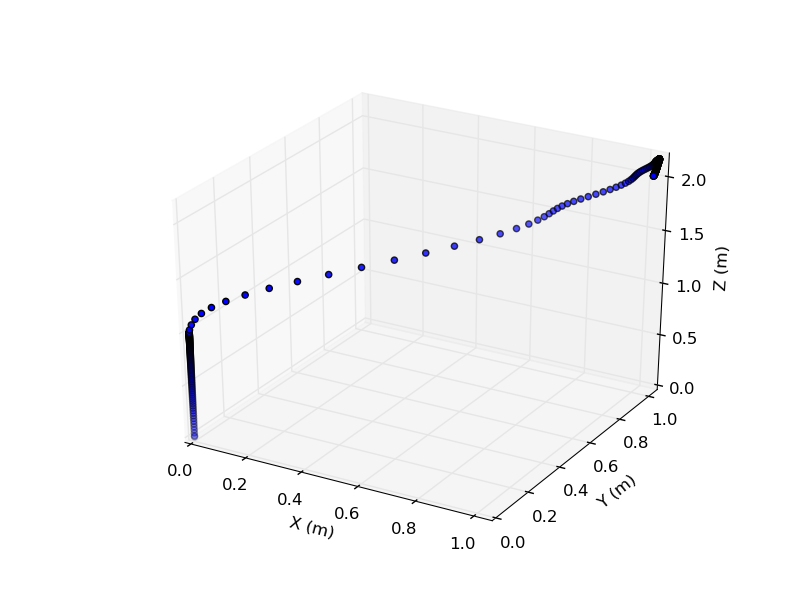
\includegraphics[width=\textwidth]{Figures/optimal_run_3D_path.png}
		\rule{35em}{0.5pt}
	\caption[Optimal Run 3D Path]{The Optimal Run - 3D path}
	\label{fig:optimal run 3D path}
\end{figure}


\begin{figure}[htbp]
	\centering
		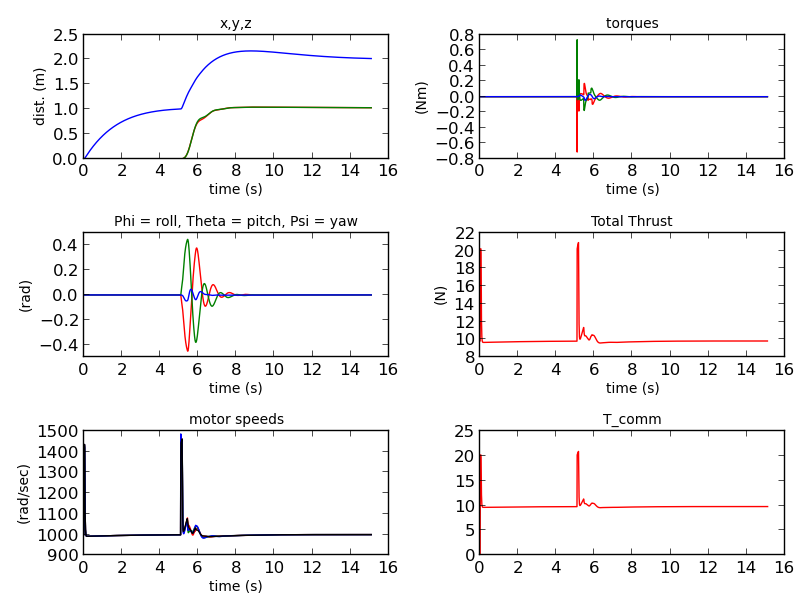
\includegraphics[width=\textwidth]{Figures/optimal_run_time_domain.png}
		\rule{35em}{0.5pt}
	\caption[Optimal Run Time Domain]{The Optimal Run - time domain}
	\label{fig:optimal run time domain}
\end{figure}



Figures \ref{fig:optimal run 3D path} and \ref{fig:optimal run time domain} show the simulation of the quad-rotor flight from the initial point $(0,0,1)$ to the desired point $(1,1,2)$ using the optimal PID tuning. There are actually two distinct legs to the simulation. The reason for this comes from the fact that there are two types of initial conditions which have fundamental differences. There is a hovering state which we use as initial conditions for the simulations in the optimization procedure. There is another mathematical state which occurs at the very beginning of the simulation. The mathematical initialization of the quad-rotor state is at the origin $(0,0,0)$ with zero velocity and acceleration but it is not exactly hovering. This subtle distinction comes from the fact that the force of gravity is not canceled out by the thrust initially. The controller has had no time to act to stabilize the system. The physical scenario that this condition would correspond to is if a person held the quad-rotor at the initial position in free space (perhaps designated as the origin) and then at $t=0$, simply let go. Another way to state this is that the simulations do not account for the normal force which would be imparted to the quad-rotor if it were simply taking off from the ground. To account for this would perhaps require augmentation of the dynamical model of the quad-rotor.

It is our aim was to start and end in a hovering state for the optimization. This is why our simulations start with a 'take-off sequence' where the quad-rotor leaves from the origin and goes to the position $(0,0,1)$. After this, the system is stabilized in a hovering state. From there, arbitrary paths can be incrementally constructed by simply redefining the desired location.

Despite the mathematical difficulties that were experienced with the various optimization techniques that were explored, this final result is useful. Until a reasonable mathematical optimization technique is found, the optimality of the solution described above is a function of how much time one is willing to run the brute force algorithm.































